\documentclass[conference]{IEEEtran}
\usepackage{graphicx}
\usepackage{amsmath}
\usepackage{amssymb}
\usepackage{subfig}
\usepackage{wrapfig}

\usepackage[font=small,labelfont=bf]{caption}

\usepackage{array}
\newcolumntype{P}[1]{>{\centering\arraybackslash}p{#1}}
\newcolumntype{M}[1]{>{\centering\arraybackslash}m{#1}}

\newcommand{\ie}{{\em i.e.}}
\newcommand{\eg}{{\em e.g.}}
\newcommand{\et}{{\em et al.~}}
\newcommand{\real}{\mathbb{R}}
\newcommand{\integer}{\mathbb{N}}

\newtheorem{theorem}{Theorem}
\newtheorem{lemma}{Lemma}
\newtheorem{corollary}{Corollary}
\newtheorem{definition}{Definition}

\DeclareMathOperator*{\argmax}{arg\,max}
\DeclareMathOperator*{\argmin}{arg\,min}

\renewcommand{\refname}{\centerline{References cited}}
\newcommand{\required}[1]{\section*{\hfil #1\hfil}}

% this handles hanging indents for publications
\def\rrr#1\\{\par
\medskip\hbox{\vbox{\parindent=2em\hsize=6.12in
\hangindent=4em\hangafter=1#1}}}

\def\baselinestretch{1}

\begin{document}

\title{\LARGE\bf %Narrow Down the Root Cause of Integrity Errors for Networked Systems
Root Cause Localization of Data Integrity Errors in Internet Scale Applications
\thanks{This work is supported by the
    US National Science Foundation through the NSF awards ACIXXX.}
}
\author{\IEEEauthorblockN{Yufeng Xin, Shih-Wen Fu, \\ Anirban Mandal, Ilya Baldin }
\IEEEauthorblockA{%RENCI\\
RENCI, UNC - Chapel Hill\\
Chapel Hill, NC, USA\\
}
\and
\IEEEauthorblockN{Mats Rynge, Karan Vahi, \\ Ewa Deelman}
\IEEEauthorblockA{%ISI\\
ISI, USC\\
Marina Del Rey, CA, USA\\
}
\and
\IEEEauthorblockN{Ishan Abhinit, Von Welch}
\IEEEauthorblockA{%CACR\\
CACR, Indiana University\\
Bloomington, IN, USA\\
}
}

\maketitle
\thispagestyle{empty}

\begin{abstract}
For large-scale distributed applications involving intensive data transfers over a network, root cause analysis (RCA) for error diagnosis becomes extremely challenging. One main reason is that the underneath network is often of multi-domain nature, where limited component level information is available, and where it is not possible to instrument and measure traffic flows at all the nodes in the network. It's hard, if not completely possible, to build proper system diagnosis models. As a result, RCA remains a guessing art that requires manual debugging and daunting amount of communication between operators from different domains and subsystems that often takes days or even weeks.  

Among the more challenging failure modes are the so-called ``grey failures" that only come to effect randomly, often at low probability. One such common failure mode is the integrity errors that may corrupt data, which is caused either by the storage subsystem or a network component along data transfer path. 

In this paper, we focus on the integrity error RCA problem in a networked system setting. We first cast it as a multi-label classification problem with the goal to enable root cause inference for a given network only from the flow level check at the end hosts. Collecting sufficient training data is fundamentally difficult with a machine learning approach, which is typical for production systems due to lack of monitoring services. We therefore built an emulation environment in a Cloud testbed that allows creating arbitrary large-scale virtual network systems. We further developed a suite of software tools to automate the training process that includes configuring the network routing, instrumenting data transfers between end hosts, injecting arbitrary integrity errors into the network components, and collecting and processing the raw data. This gives us extra benefits in experiment repeatability and efficiency. For evaluation, we trained several multi-label classification models and validated their performance with a Top-$k$ accuracy metric for an emulated network. The results demonstrate the efficacy of the approach and potential to apply the learned models to production systems.  

\end{abstract}

\section{Introduction}
\label{sec:introduction}
Root cause analysis (RCA) is a critical function in operating and managing complex networked systems, be it physical, software, or hybrid~\cite{RCA-Review-2017}.
It aims to identify the component(s) and process(es) responsible for the fault manifested by the wrong results or system failures in a timely fashion.
Traditional RCA relies on system domain models that can be used to deduce the potential component failures from the system symptoms and behaviors.
However, exponentially increasing system scale, complex component interdependencies, and lack of visibility in multi-domain, large-scale networks have 
significantly made it harder to build such models for efficient fault identification and localization for modern distributed systems. 
As a result, RCA in such a distributed and opaque system setting has drawn extensive research attention in recent years, which have found prominent uses
 in data center networks and Internet applications. Not surprisingly, these studies have adopted the machine learning (ML) or data analytic approaches
due to the relaxed requirements on accurate domain models~\cite{netbouncer:nsdi18,Link-JIoT-2019}.

In this paper, we take a new application domain, the scientific workflow management systems (WMS), as our primary motivating use case to tackle the complex
 system RCA problem using a machine learning approach. WMS facilitates in-order execution of jobs in workflows and includes large amounts of interdependent
  data transfers, storage functions, and computation tasks. These tasks are often distributed over distributed hardware, software, and data resources
   located in different facilities nationwide or globally. Inevitably, frequent system failures and reliability issues 
caused by errors and faults from underlying subsystems have been serious concerns for the WMS community. 
Therefore most WMS have built-in failure handling mechanisms like redundancy and automatic retries. 
They also try to provide as much log information as possible to help with failure diagnosis, which normally assumes a long manual process.

Since a typical workflow system runs as a middleware sitting several layers above the infrastructure resources that are managed 
and operated by different service providers (domains), it has a limited view of the health of the infrastructure components. 
Most critically, it has no direct knowledge of the exact path of the data movement,
sometimes even the sources and sinks are normally abstracted in virtual namespaces.  
Consequently, fault diagnosis, especially identifying the root cause of the failures becomes extremely difficult, and normally 
costs coordinated efforts and long hours from many operators of different sub-systems, often after many unsuccessful (and wasted) retries from the users. 
Hence, analyzing the root cause of failures for data integrity errors in distributed workflow executions is a representative yet very difficult problem.

In a nutshell, ML-based RCA can be formulated as a multi-class classification problem, where the potential root causes are the labels and various 
measurement and observations of the tasks and data flow level observations are used as the features.
RCA for large-scale networked systems poses other unique challenges in adopting ML approaches.
 
The first challenge comes from the prevalence of so-called {\it gray failures} in the networked system, in addition to the normal {\it stop failures}~\cite{GrayFailure:2017,DeepView:NSDI18}. A {\it stop failure} is a kind of hard failure, which refers to the complete breakdown of a component that disrupts all traffic flows or paths over this component deterministically~\cite{Link-JIoT-2019}. {\it Gray failures} are those probabilistic failures in a component that would act normally most of the time and that could not be caught by the traditional deterministic system monitoring and diagnostic tools. We categorize two types of  {\it gray failures}: performance degradation and data integrity errors. The former is normally caused by system overload that will lead to slow response, timeout, and the frequent reboot of the servers or software. The latter may randomly corrupt bits in a block of data or packets over network transfer. Since existing checksum mechanisms implemented in TCP and the storage services are not sufficient to guarantee end-to-end data integrity, they often get unnoticed for a long time until severe consequences to applications occurred. Therefore modern WMS have started to add end-to-end integrity check mechanisms, including in Pegasus~\cite{swip:pearc:2019} and Globus~\cite{IntegrityVerification:DataTransfer}.

The second challenge lies in the difficulties in acquiring sufficient training data feeds to a ML-based RCA system. For a system over the Internet, the global routing information is not completely available for the RCA system as they are normally proprietary to the different service providers (domains). The possible monitoring data sources or active probe sites in a network are always limited. As a result, in addition to passive monitoring data, active probes or event fault injections are often used to generate more diagnosis data~\cite{active:iot:2019, NetPoirot:Sigcomm2016}. Then, due to the desire of conducting RCA in real-time, how to minimize the overhead and latency of data collection in a production setting becomes a significant design issue.

The last but not the least challenge is to design and train the right ML models to achieve high diagnosis accuracy, out of a large pool of candidates~\cite{Boutaba:2018aa}. We will show that even the most basic questions of defining a data point, feature selection, and performance evaluation need special consideration.

In~\cite{Link-JIoT-2019}, the authors attempted to identify the stop failure of network links via the popular multi-class ML models using end-to-end passive traffic engineering measurements (throughput, latency, and packet loss). The authors in \cite{DeepView:NSDI18} took an active probe approach to localize the fault in a virtual disk system to the finest granularity up to the network switches. In~\cite{netbouncer:nsdi18}, a necessary condition was derived on the minimal set of paths that active probes need to be sent over the targeted network. The line of work including~\cite{NetPoirot:Sigcomm2016,KDD14} adapted a statistical learning approach to infer the probabilistic relationship between the path failure and the link faults. All these research works made a strong assumption that one can instrument probes or observations from any node to any other node in the network since their target systems are data center networks that they own. In an earlier study, the decision tree model was used to predict if a request will fail or succeed over a flawed network system~\cite{DT:2004}. Bayesian inference was demonstrated to be efficient for fast diagnosis when the causal relationship model is established in a large Internet system~\cite{BN-Internet:2007}.

In this paper, we first cast the WMS integrity error diagnosis as a networked system Root Cause Analysis (RCA) problem, where limited network system information is available for end-to-end data transfers (Section~\ref{sec:integrity}). Our main hypothesis is that the mapping between the endhost level flow statistics and the possible network component failures can be learned and inferred from a sufficiently large amount of labeled training data. In order to obtain sufficient training data and make repeatable experiments more efficient, we created an experimental system in a Cloud testbed that can automatically create a large-scale OSPF-enabled virtual network system, initiate data transfers between end hosts, and inject arbitrary integrity errors into the virtual router interfaces and end hosts (Section~\ref{sec:emulation}). We then studied several variants from three different families of multi-class classification models, Bayesian inference, SVM, and Decision Tree, and validated their accuracy performance using a Top-$k$ accuracy metric (Section~\ref{sec:ml}). With the data collected from the emulation, we evaluate their accuracy in Section~\ref{sec:evaluation}. We specifically studied the impact of available data transfer data in terms of end host pair coverage. We conclude the paper with our future research plan in Section~\ref{sec:future}.


\section{A Network Failure Localization Model}
\label{sec:fault}
In this section, we present the inference model to localize the failures based on the path level measurements. 
~\ref{fig:example} shows a simple example network we target in this paper. It consists of several sites interconnected by a network cloud 
where only the network nodes and their interfaces are known (otherwise the failure localization is meaningless). 
A distributed application will incur traffic flows along an unknown path between pairs of end hosts. These flows are subject to 
the measurement of the applications to test if they are corrupted. Two such flows, $c3-d2$ and $c2-d4$ are shown in the figure. Intuitively, 
if both flows suffer from data corruption, the interface with the cross mark in Node $N2$ should be inferred to be the culprit.   

\begin{figure}
  \begin{center}
    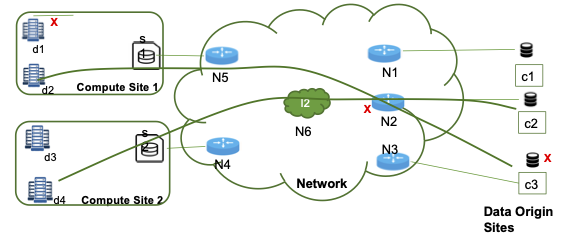
\includegraphics[width=0.48\textwidth]{./figure/example_network.png}
  \end{center}
\caption{An Example Network}
\label{fig:example}
\end{figure}

In most existing work on in gray failure localization, the network is modeled as a simple graph $G(V,E)$  
with a set of nodes $V$ connected by a set of links $E$. The following bipartite mapping 
formula was used to capture the relationship between the link failures and the path level measurements~\cite{netbouncer:nsdi18,DeepView:NSDI18,arzani2018democratically}. 
The failure being considered is packet loss. 
The reasonings behind these models are similar: due to scalability or privacy constraints, 
monitoring every component of interest in a large-scale network is 
not feasible, while the path level measurement is more practical to deploy and instrument.  
\begin{flalign}\label{eq:prob}
\begin{aligned}
&P(No\ Failure\ in\ Path \ i) = \\
&\prod_{j \in Path\ i}P(component\ j\ is\ normal)
\end{aligned}
\end{flalign}
This can be transformed to a familiar linear regression model for every identifiable path in the network after taking log on the equations.
\begin{flalign}\label{eq:linear}
\begin{aligned}
&p_i = &\sum_{j \in Path\ i} c_j\ & \forall i \in P
\end{aligned}
\end{flalign}
Here $P$ represents the set of paths that are measured and a fundamental assumption underscoring these models is that routing of every path 
in $P$ over link set $E$ needs to be obtained. In addition, it was also assumed the measurement system have the access to all network nodes 
to instrument path measurements, \ie, the source and destination of a path can be any nodes. In summary, to 
establish the regression model to obtain satisfactory inference performance, 
substantial efforts were made to (i) identify the routing of the paths, (ii) determine the path set for good coverage, and 
(iii) enable constant measurement of paths. Then the path measurements ($p_i$) will be obtained to estimate the link error probability ($c_j$) using this model.

In our wide-area multi-domain network setting, as we discussed in an earlier work~\cite{iris:ictc21}, it is not practical to identify the routing of 
the paths over the network and even the network topology beforehand. This means that it is difficult to establish a model like Eq. (\ref{eq:linear}). 
We also can not assume access to nodes in the network domains to instrument or measure paths.  

We thereafter distinguish between application end hosts (that generate and receive data) and networking devices (routers or switches), 
\ie, $V$ includes $H$ end hosts and $R$ routers. And we redefine $E$ to be the set of network components where failures are supposed to be 
localized, specifically all the network interfaces on $V$ and the end hosts $H$. We further constrain that only passive path measurements are available from certain applications on the end hosts, \ie, $P$ in our system only consists of paths originating from and ending in end hosts in $H$, which implies a much smaller identifiable path set. In the example network Fig.~\ref{fig:example}, none of the network nodes, $N1, \ldots, N6$, can be the source or destination of a path. And for a path between two end hosts, its routing is unknown. The only knowledge our model has is the bag of nodes and their interfaces for traffic forwarding.  

We further observe that one component failure (e.g., $x_j$) 
could cause multiple paths erroneous while one erroneous path may be the result of a failure at different components. The standard model Eq. (\ref{eq:linear}) ignores 
the correlation between multiple paths sharing a common component. We thereafter inverse the equations to represent the component failure probability as a function of 
the path failure probabilities as the following prediction model. 
 
\begin{flalign}\label{eq:inverse}
\begin{aligned}
Y = F(x_1, \cdots, x_p, \cdots, x_{|P|} ) \\
 = \sum_{p \in P} w_p x_p +w_0
\end{aligned}
\end{flalign}

Specifically, $Y$ represents a vector space $(y_1, \ldots, y_v, \ldots, y_{|V|)}$ where $y_v$ represents the failure probability of component 
$v \in V$.  $X = (x_1, \ldots, x_p, \ldots, x_{|P|})$  forms the feature space that is defined by the combinations of the path failure probability. 
As shown in Eq. (\ref{eq:inverse}), we can further make it a linear regression model, which produces excellent performance as we will show in 
the evaluation section. We note, unlike in the existing work where failure localization is on network links, the network components in our model 
are the nodes and their interfaces because we assume the network topology is unknown.

Since any component failure only affects a small number of paths that go through it, plus multiple simultaneous failures are rare in reality, it is 
reasonable to expect both the feature matrix and the coefficient matrix is sparse, representing the samples collected during one inference 
window. This suggests using the regularization technique to make most of the estimated coefficient to be zero. The most efficient technique 
to achieve this intention is to add a L1-norm constraint is known as Lasso~\cite{DeepView:NSDI18}, where the regression optimization objective 
is defined as:    

\begin{flalign}\label{eq:lasso}
\begin{aligned}
\hat{W} =  \argmin_{W \in R^{|P|}}\vert\vert{\textbf{Y}-\textbf{X}W}\vert\vert _2^2 + \lambda \vert\vert{W}\vert\vert_1
\end{aligned}
\end{flalign}

Here $\textbf{Y}$ and $\textbf{X}$ are the sample matrix. This technique has proven extremely efficient in dealing with overfitting. 
The vector definition of $Y \in R^{|C|}$ means for each sample $n$, all entries but one in $Y^n$ are zeros. 
Compared to the scalar variable of a specific component failure probability, this multi-output model 
captures the independence between all the failures and would help the training and prediction quality.  










\section{Missing Data and Imputation}
\label{sec:sl}
As we discussed in Section~\ref{sec:introduction}, missing data is pervasive in reality due to lost or unavailable measurement data. 
It means that some samples, in the training set or the test set, have missing features. 
Using the example network in Fig.~\ref{fig:example} to illustrate, during a diagnosis time window, the application may not incur traffic between 
$c1$ and $d1$, or it never needs to transfer data between the origin sites, or the application measurement system may corrupt or lose some 
measurement data for some traffic flow. All these will lead to 'holes' in the feature columns in the data sets. In the first two cases, 
entire feature columns will be missing in our model~\ref{eq:inverse}.

Missing data can be categorized into three types: (i) the data is missing completely at random (MCAR) if the missingness does not depend 
on any of the observed and unobserved variables, (ii) the data is missing at random (MAR) if the missingness is dependent only on the observed variables, 
(iii) the data is missing not at random (MNAR) if the missingness is neither MCAR nor MAR, \ie, the missingness depends on both observed variables and the 
unobserved variables. The majority of existing studies used the MCAR assumption~\cite{Yoon2018GAINMD}. 

There are many kinds of missing data recovery methods commonly used in the literature. These methods largely fall into three categories.

The {\it univariate} methods impute values in a  feature dimension using only non-missing values in that feature dimension. It simply replaces the missed 
values with certain statistics of the non-missing values such as the zero, mean, median, mode, max, or min. 

The {\it multivariate} imputation algorithms use the entire set of available feature dimensions to estimate the missing values based on the assumption 
of correlations between the feature dimensions. Each feature with missing values is modeled as a function of other features, and therefore the imputation itself 
is modeled as a regression problem that is trained and used to estimate the imputation. In order to achieve the best performance, especially to avoid the 
overfitting from certain features, it is conducted in a series of regression iterations: at each step, a feature is used as the output of other features and the resulted model is used to estimate the missing feature. After all features are processed or the designated max iteration is reached, the results of the final estimation are used to impute 
the missing data.

Our prediction model in Eq.~(\ref{eq:inverse})  uses the path (flow) measurements as the input. It naturally fits the multivariate imputation approach 
because the path failures caused by a common component failure are correlated. In contrast, the existing models based on Eq.~(\ref{eq:linear}) use the 
component failure as the input variables that are independent of each other. The {\it multivariate} imputation does not seem to make sense.
The {\it univariate} method is deemed not applicable due to the sparse nature of the feature matrix and lack of reasonable explanation.

Most recently,  the Generative Adversarial Nets ({\it GAN)} framework has shown good performance to generate the missing data.
In this model, the generator’s goal is to accurately impute missing data, and the discriminator’s goal is to distinguish between observed and imputed 
components. The discriminator is trained to minimize the classification loss (when classifying which components were observed and 
which have been imputed), and the generator is trained to maximize the discriminator’s misclassification rate. Thus, these 
two networks are trained using an adversarial process~\cite{Yoon2018GAINMD,Awan2021ImputationOM}.

There are off-the-shelf libraries that support both univariate and multivariate imputations in popular software packages like R and 
Scikit-learn~\cite{JSSv045i03,10.1371/journal.pone.0254720}. The imputation can also be performed multiple times with different 
random number seeds to generate multiple imputations. This is important if the statistical analysis is needed, \eg, in the medical domain. 

Most of existing missing data studies focus on minimizing the imputation errors of the data in the feature space. However the ultimate goal 
is the performance of the prediction models after missing data is imputed.

Corresponding to our model in Eq.~(\ref{eq:inverse}), missing data will cause values of some $x_p$ to be null. 
The feature space is defined in a $|P|$-dimensional space $\mathbf{X} = \mathbf{X_1} \times \ldots \times \mathbf{X_{|P|}}$. 
Following the MCAR assumption 
on the missing data, we can define a mask vector $M = (M_1, \ldots, M_{|P|})$ taking random values in ${(0, 1)}^{|P|}$.  
A sample vector $X = (X_1 \times \ldots \times X_{|P|})$ 
can be masked by $M$ to generate a corresponding sample vector with missing data $\tilde{X} = \tilde{X}_1 \times \ldots \times \tilde{X}_{|P|}$ as follow:

\[
\tilde{X_p} = 
\begin{cases}
  X_p & \text{if $M_p = 1$} \\
  null & \text{otherwise}
\end{cases}
\]

From an arbitrary missing rate $r \in (0, 1)$, a random mask vector $M_r$ can be created to emulate missing data from a given feature matrix $X$. 
For a particular missing feature $X_r \in X$, the imputation essentially creates a regression model that makes $X_r$ the output variable and all the 
other features the input variables.   

\begin{flalign}\label{eq:imputation}
\begin{aligned}
X_r = F(x_1, \cdots, x_p, \cdots, x_{|P|} ), \ p \neq r \\
\end{aligned}
\end{flalign}

At the end of the imputation, a recovered data set $\hat{X_r}$ is generated. The goal is to make these as close as possible.

Our main results are based on the MCAR missing data model, the {\it multivariate} imputation algorithms, and regularized regression model, 
which can be summarized in the following pipeline definition with Scikit\_Learn.
%~\cite{Scikit:web}. 
\begin{verbatim}
    estimator = make_pipeline(
        IterativeImputer(random_state=0, 
        		missing_values=np.nan, 
        		estimator=impute_estimator),
        PolynomialFeatures(poly),
        br_estimator
    )
\end{verbatim}

In the pipeline, the {\it impute\_estimator} specifies the regressor for missing data imputation and the {\it br\_estimator} specifies the regressor to infer the 
localized failure probability. We added a {PolynomialFeatures} element to evaluate if polynomials of higher degree perform better than the linear regressor.

This pipeline construct allows us to systematically evaluate the performance of multiple regressors in both {\it impute\_estimator} and {\it br\_estimator}, as well 
as tuning their hyperparameters. As we discussed earlier, in theory, Lasso should be a suitable regressor in both places. We also evaluated other popular 
regressors that include Ridge, BayesianRidge, ExtraTreesRegressor, and KNeighborsRegressor.



 


\section{Experiments and Evaluation}
\label{sec:evaluation}
We created the topology shown in Figure~\ref{fig:topology} in ExoGENI to conduct our experiments. Among the $23$ nodes in this topology, we specify $6$ data origins and $6$ data sinks as the end hosts to transfer a batch of data files ($886$ files) of different sizes that we randomly acquired from OSG. There are $49$ links in total with which we try to emulate a topology following the power law, i.e., $4$ routing nodes in the middle to emulate the backbone domain and the rest emulate the access domains in between the backbone nodes and the end hosts. 

We ran two sets of experiments to collect two sets of training data. In the first one, called {\it Partial},
data transfers only happen between the origins and sinks. In the second one, called {\it Complete}, 
data transfers happen between all the end host pairs. Each origin node sends all the $886$ files to all the receiving nodes, where the file integrity is being checked.

For each experiment, probabilistic integrity error or network impairment via the Chaos Jungle tool is injected to the links and end hosts in sequence with the given probability setting. For each fault injection scenario, the entire set of {\it Partial} or {\it Complete} data transfers are conducted. The receiving node checks if the receiving file is identical to the original copy and marks the data transfer as failure if files are not identical. A file could also be missed which is treated as failure. We treat retransmission as a separate feature. Each link or node component with fault injected is a label and each file transfer becomes a data point in the training set. We further parallelized the data transfer process to reduce the emulation time down to about twenty four hours for this particular network. 

Following figures show the accuracy results. The figures from Decision Tree and Bayes models have two parts: the left part shows the results for the {\it Partial} data set and the right part shows the results for the {\it Complete} data set. Each part depicts four levels of accuracy: flow, top-1, top-2, and top-3. The results from the SVM show two different types of models: linear SVM and general SVM with RBF kernel.
We inject integrity errors in $67$ network components including the interfaces and end host nodes, which represents $67$ labels. As a very basic benchmark, the accuracy of random classification is merely $\frac{1}{67}$.
\begin{figure}[!ht]
\begin{center}
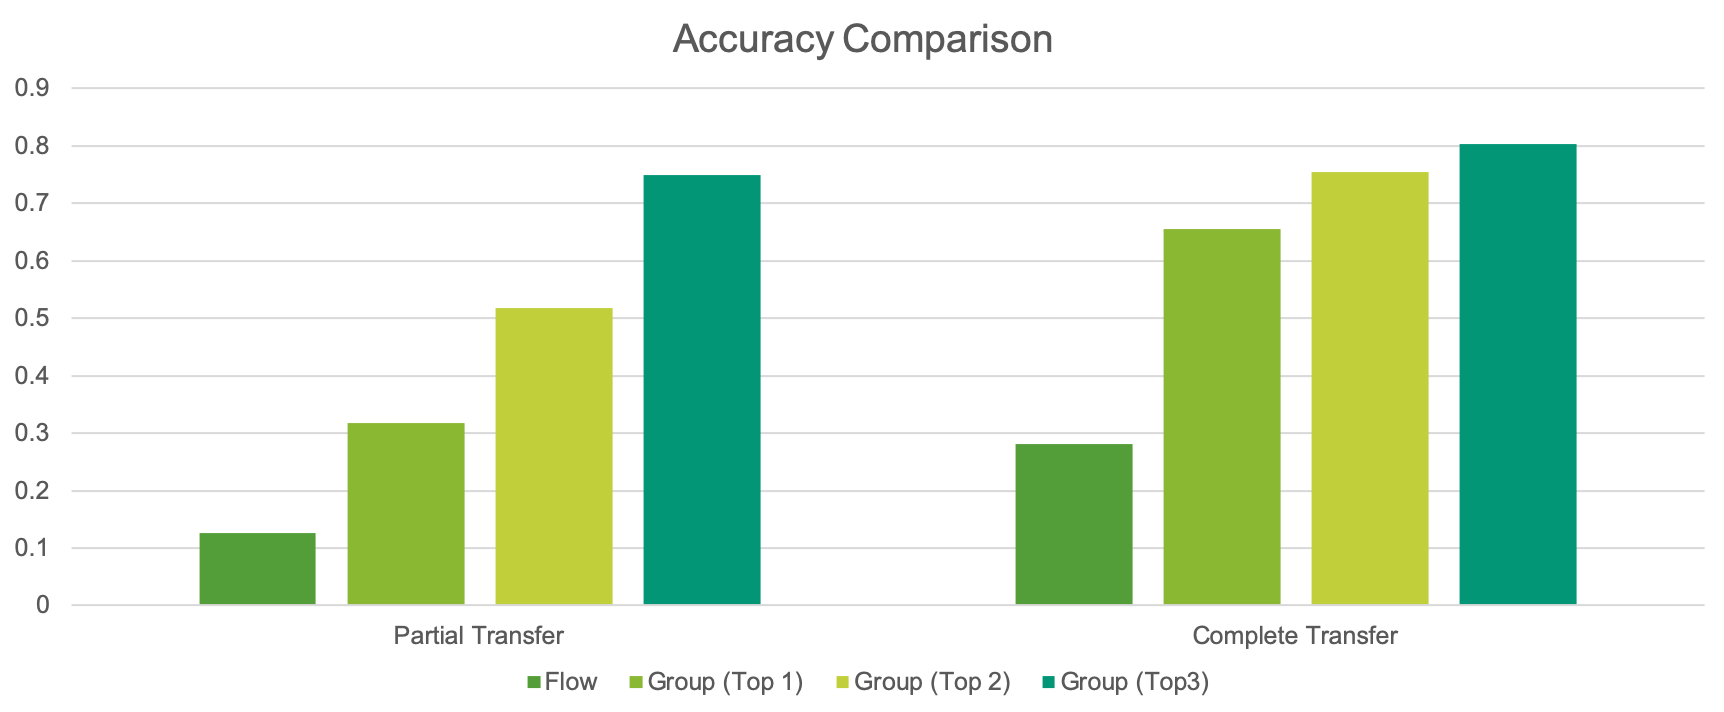
\includegraphics[width=0.45\textwidth]{./figure/dt-result}
\end{center}
\vspace{-0.05in}
\caption{Classification Accuracy with Decision Tree Model}
\vspace{-0.05in}
\label{fig:dt}
\end{figure}

Fig.~\ref{fig:dt} presents the results using the random forest model. The single flow level accuracy is very poor and the accuracy increases dramatically with bigger $k$. It also clearly shows that the model with {\it Complete} data performs much better than the {\it Partial} case. However, the gap becomes small when $k=3$. 

\begin{figure}[!ht]
\begin{center}
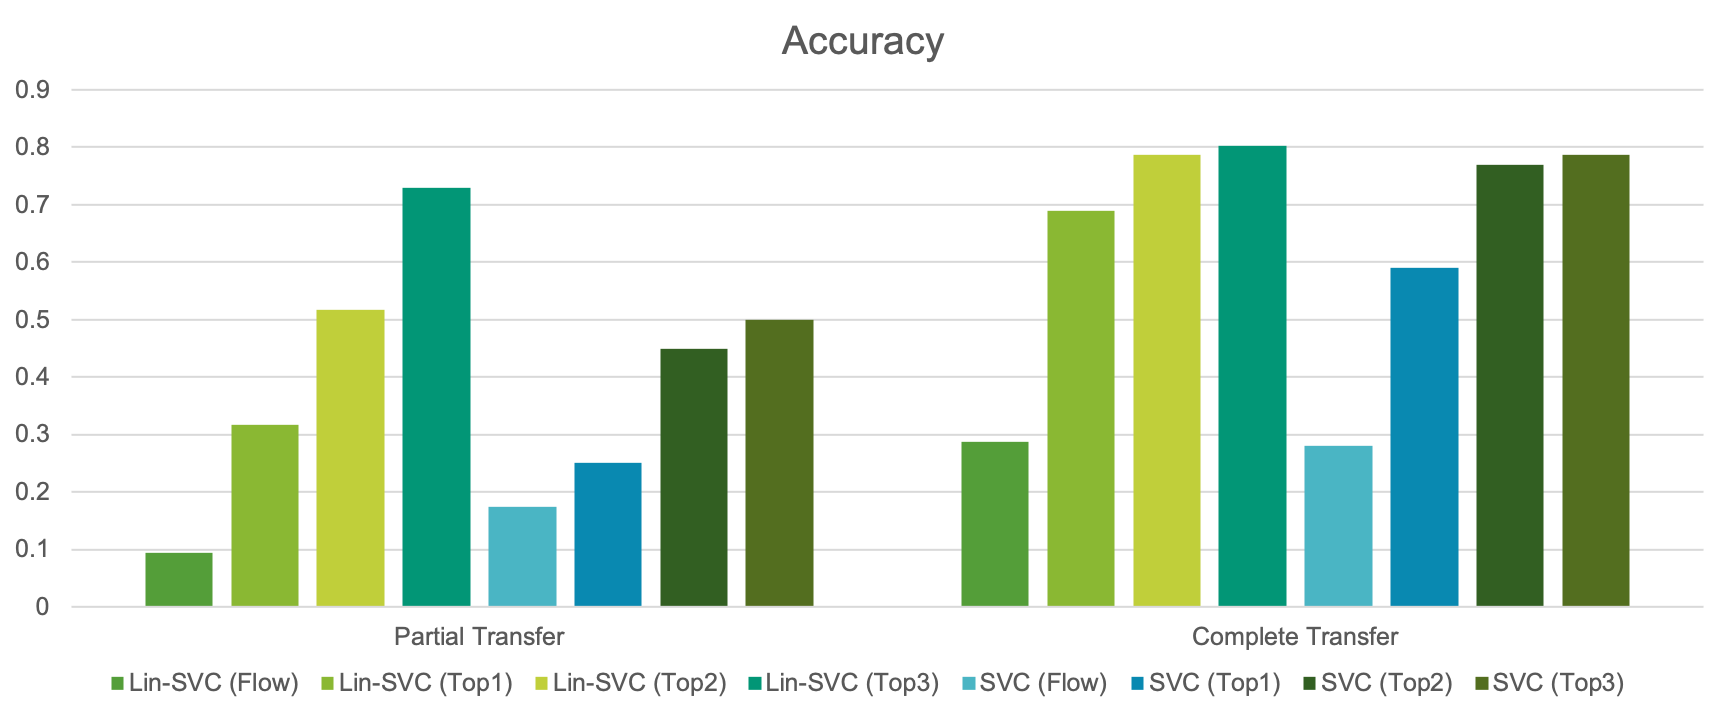
\includegraphics[width=0.45\textwidth]{./figure/svm-result}
\end{center}
\vspace{-0.05in}
\caption{Classification Accuracy with SVM Model}
\vspace{-0.05in}
\label{fig:svm}
\end{figure}

Fig.~\ref{fig:svm} depicts the results using two different models: linear and general SVM with RBF kernel. It shows the same trends with regards to $k$. It also clearly shows that Linear SVM performs better than the general SVM.
\begin{figure}[!ht]
\begin{center}
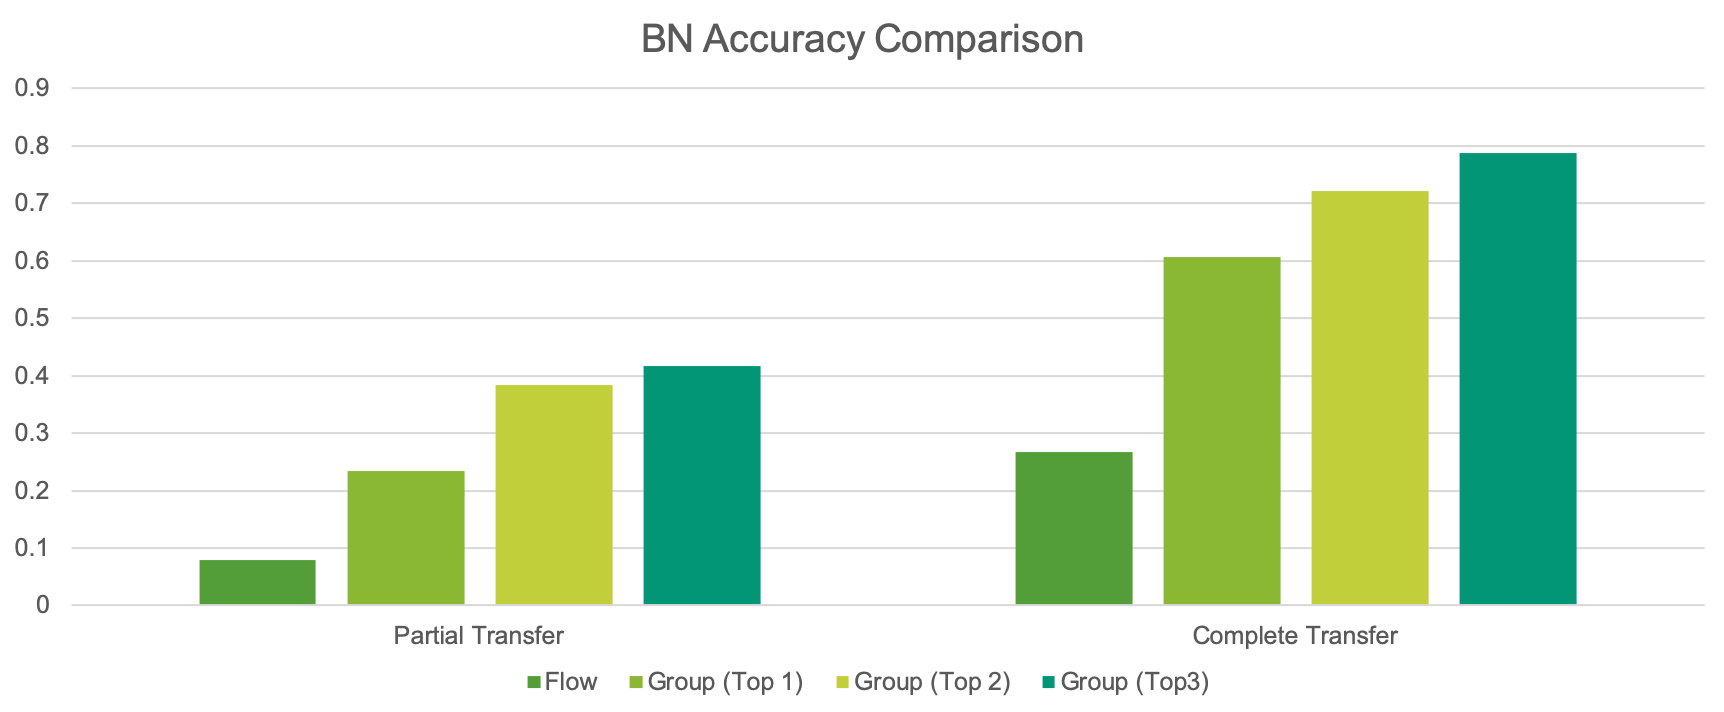
\includegraphics[width=0.45\textwidth]{./figure/bn-result}
\end{center}
\vspace{-0.05in}
\caption{Classification Accuracy with Multinomial Naive Bayes}
\vspace{-0.05in}
\label{fig:bn}
\end{figure}

Fig.~\ref{fig:bn} shows the results using the Multinomial Naive Bayes approach. Again, the accuracy increases with $k$.

When comparing between above three models, the random forest performs the best, linear SVM the next best, and the Bayes model performs the worst. 

When $k=3$, the maximal achieved accuracy is slightly above $80\%$, which is very promising for our specific network RCA problem. We tried larger values of $k$. The accuracy doesn't change much until $k$ reaches 20, when it will jump to above $90\%$. We believe the accuracy stall may be mainly due to the particular topology and more importantly the set of the end hosts for data transfers that do not include all the router nodes, which violates the necessary condition to cover all the possible failure causes in a network~\cite{netbouncer:nsdi18}.  

We next look into the training time of the above three models. From Table.~\ref{tab:time}, it is clear that SVM takes significantly longer time than the other two. Actually the SVC with the default RBF kernel takes much longer time than the linear SVC whose running time is shown in the table. Between the other two, the decision tree model takes the shortest time. Another observation is that the training with the {\it Complete} data set finishes much faster than that with {\it Partial} data set. This makes sense because more complete training data helps the model training converge faster. 

To make the evaluation complete, we also present the F-Score for the single label classification {\it Complete} case in the same table. The SVM model gets the best F-score. As we stated before, we believe the accuracy is the more meaningful metric for the RCA problem, though we will continue to explore better metrics.     
\begin{table}[!ht]
\caption{Training Time and F\-Score
\label{tab:time}}
\vspace{-0.1in}
\begin{center}
\begin{tabular}{ |c|c|c|c| } 
 \hline
  & Partial & Complete & F-Score ($k=1$)\\ 
 \hline\hline
 Decision Tree & 164ms & 95.1ms & 0.3266\\ 
 \hline
 Bayes & 416ms & 174ms & 0.3382 \\
 \hline
 SVM & 26700ms & 10300ms & 0.368 \\ 
 \hline
\end{tabular}
\end{center}
\vspace{-0.1in}
\end{table}
Combining both training accuracy and training time, the random forest model appears to be a clear winner for the studied RCA problem.

\section{Conclusions and Future Work}
\label{sec:future}
We developed a machine learning based network integrity error RCA system that leverages the end-to-end flow monitoring information 
from the application layer, augmented by limited network information. The impacts of different combinations of numerical and categorical data 
features under different realistic network and measurement assumptions on the inference accuracy are quantified via an emulated network created 
in an automated high-fidelity emulation environment we built. The analysis validated that high RCA accuracy to the device level can be achieved with an efficient supervised 
learning model even when only partial network and flow level measurement information are available.

For our future work, we plan to study networks of larger scale with different topology characteristics, more finely tuned ML models, and possible integration with limited network monitoring information. We will further explore the multi-granularity classification framework for large networks. While we focused on single faulty component scenario for integrity errors in this study, we plan to expand to other failure modes and performance degradation RCA systems with multiple concurrent faults. We will also study stochastic approaches that leverage the probability distribution characteristics of the network failures.  


\bibliographystyle{IEEEtran}
\bibliography{iris_sl,iris}

%\newpage
%\begin{appendix} 
%\hfill \break

{\LARGE Demo Description}\\

In order to obtain sufficient amount of training and test data, while guaranteeing experimental repeatability and efficiency, we created a suite of software tools to automate emulation experiments in a Cloud testbed, which can automatically create a large-scale OSPF-enabled virtual network system, initiate data transfers between end hosts, and inject arbitrary integrity errors into the virtual router interfaces and end hosts.  

Our main design objectives is to automate the experiment creation, configuration, and data collection at any given scale. This not only guarantees repeatable experiments at different scales, but also makes data manipulation for ML model training for RCA much more efficient.   

We will demonstrate the three main components of the emulation and RCA analysis system. An emulation experiment in ExoGENI testbed is depicted in Fig.~\ref{fig:chaosjungle}.

\subsection{Network creation and configuration}
An arbitrary topology can be created with nodes in the form of virtual machines (VM) running customized images. We leverage the Postboot scripting capability offered by ExoGENI testbed to automate the network configuration.  

In our experimental topology, we use a set of end hosts to emulate the OSG data sources and sinks, a virtual network consisting of core routers emulating the backbone network service providers (Internet2, ESNet, etc) and access routers emulating the access network service providers (regional research and education networks and campus networks). All nodes are connected with virtual layer-2 links with certain throughput guarantee as the private data plane. An extra management plane interface is also available on every node, which provides remote access from the public Internet. The end hosts run an Ubuntu image with our Chaos Jungle fault injection tools. The routers run an Ubuntu image with the Zebra software router and our Chaos Jungle fault injection tools.

At the virtual node booting time, our customized Postboot scripts automate the following steps: (1) detect all the interfaces and their IP addresses, and all the neighboring nodes and the links; (2) create the configuration files for Zebra and OSPF daemons and start the routing control plane at the router nodes; (3) detect and add the default routes at the end host nodes.    

ExoGENI provides an API to launch any given experimental topology. On a successful execution, our experimental topology will be up and running with routing configured and network reachability established among all end hosts.   

\subsection{Data transfer and fault injection}
For every experiment, we attach a controller node that can reach all the nodes in the topology via the management plane interface. The controller is provided a Postboot script that automatically learns the experimental topology, creates a list of end hosts, routers, and links, and populates the end hosts with a set of files for the data transfer.

A user can log into the controller node, modify the experimental configuration files that define the data origin and sink nodes, the list of nodes to introduce storage integrity error, the list of network link interfaces to be disrupted by the Chaos Jungle tool, and the fault injection probability.

Then the experiment software can be started to inject the fault, transfer the data files from the origins, check the integrity at the sinks, and collect the data. This sequence is repeated for every fault specified in the configuration file.

\begin{figure}[!ht]
\begin{center}
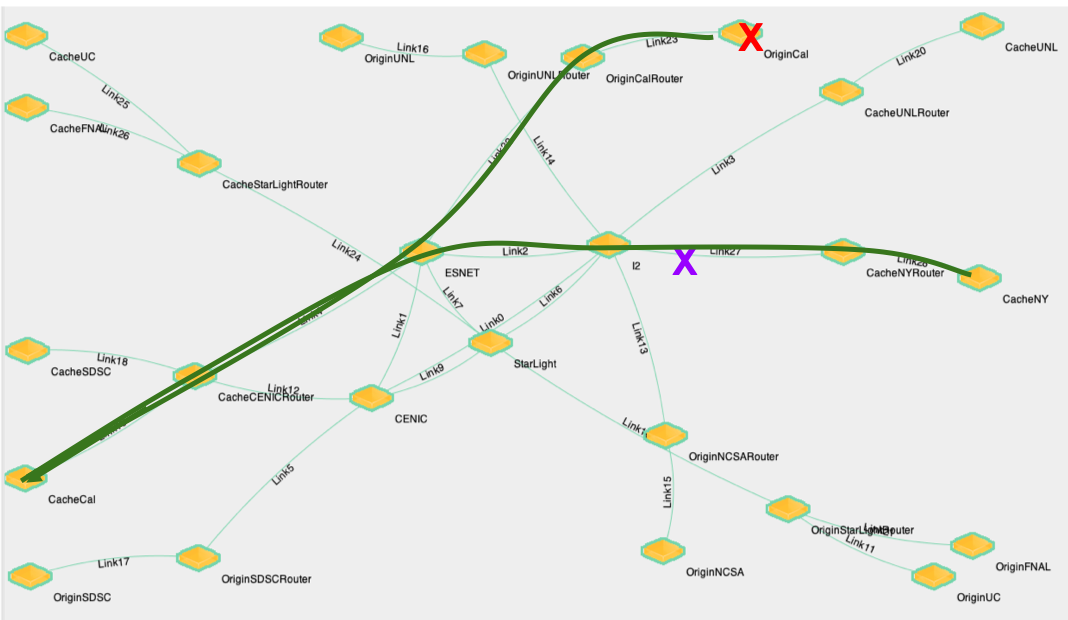
\includegraphics[width=0.48\textwidth]{./figure/ChaosJungle}
\end{center}
\caption{Network Emulation and Integrity Error Injection in ExoGENI}
\label{fig:chaosjungle}
\end{figure}

\subsection{Data collection and analysis}
At the last step, all the raw data will be processed and stored in final result database files with predefined feature columns. Each database entry represents one data transfer with features of file name, file size, origin, sink, access router, integrity error or not, etc. However, the forwarding path is unknown as it is controlled by the routing control plane process. The final result is exported to a Jupyter notebook environment where machine learning based data analysis is performed.

\hfill \break

{\LARGE Demo Set-Up}\\

The default display set-up plus Internet access is sufficient for our demonstration needs as we only run the client at the demo site. The actual experiments will be run in the remote Cloud.


%\end{appendix} 

% That's all folks!
\end{document}
